\documentclass{standalone}

\usepackage[T1]{fontenc}
\usepackage[utf8]{inputenc}
\usepackage{eulervm}
\usepackage{amsmath}
\usepackage{bm}
\usepackage{tikz}
\usepackage{environ}

\usetikzlibrary{fit}
\usetikzlibrary{patterns}
\usetikzlibrary{arrows}

\usepackage{color}

\definecolor{Comment}{RGB}{97,161,176}

\definecolor{btfGreen}{RGB}{51,160,44}
\definecolor{btfRed}{RGB}{190,60,90}

\definecolor{bleuUni}{RGB}{0, 157, 224}
\definecolor{marronUni}{RGB}{68, 58, 49}
\definecolor{grayMarronUni}{RGB}{60, 60, 60}
\definecolor{grayBleuUni}{RGB}{118, 118, 118}

\definecolor{bluecite}{HTML}{009DE0}

\definecolor{Paired-2}{RGB}{166,206,227}
\definecolor{Paired-1}{RGB}{31,120,180}
\definecolor{Paired-4}{RGB}{178,223,138}
\definecolor{Paired-3}{RGB}{51,160,44}
\definecolor{Paired-6}{RGB}{251,154,153}
\definecolor{Paired-5}{RGB}{227,26,28}
\definecolor{Paired-8}{RGB}{253,191,111}
\definecolor{Paired-7}{RGB}{255,127,0}
\definecolor{Paired-10}{RGB}{202,178,214}
\definecolor{Paired-9}{RGB}{106,61,154}
\definecolor{Paired-12}{RGB}{255,255,153}
\definecolor{Paired-11}{RGB}{177,89,40}
\definecolor{Accent-1}{RGB}{127,201,127}
\definecolor{Accent-2}{RGB}{190,174,212}
\definecolor{Accent-3}{RGB}{253,192,134}
\definecolor{Accent-4}{RGB}{255,255,153}
\definecolor{Accent-5}{RGB}{56,108,176}
\definecolor{Accent-6}{RGB}{240,2,127}
\definecolor{Accent-7}{RGB}{191,91,23}
\definecolor{Accent-8}{RGB}{102,102,102}
\definecolor{Spectral-1}{RGB}{158,1,66}
\definecolor{Spectral-2}{RGB}{213,62,79}
\definecolor{Spectral-3}{RGB}{244,109,67}
\definecolor{Spectral-4}{RGB}{253,174,97}
\definecolor{Spectral-5}{RGB}{254,224,139}
\definecolor{Spectral-6}{RGB}{255,255,191}
\definecolor{Spectral-7}{RGB}{230,245,152}
\definecolor{Spectral-8}{RGB}{171,221,164}
\definecolor{Spectral-9}{RGB}{102,194,165}
\definecolor{Spectral-10}{RGB}{50,136,189}
\definecolor{Spectral-11}{RGB}{94,79,162}
\definecolor{Set1-1}{RGB}{228,26,28}
\definecolor{Set1-2}{RGB}{55,126,184}
\definecolor{Set1-3}{RGB}{77,175,74}
\definecolor{Set1-4}{RGB}{152,78,163}
\definecolor{Set1-5}{RGB}{255,127,0}
\definecolor{Set1-6}{RGB}{255,255,51}
\definecolor{Set1-7}{RGB}{166,86,40}
\definecolor{Set1-8}{RGB}{247,129,191}
\definecolor{Set1-9}{RGB}{153,153,153}
\definecolor{Set2-1}{RGB}{102,194,165}
\definecolor{Set2-2}{RGB}{252,141,98}
\definecolor{Set2-3}{RGB}{141,160,203}
\definecolor{Set2-4}{RGB}{231,138,195}
\definecolor{Set2-5}{RGB}{166,216,84}
\definecolor{Set2-6}{RGB}{255,217,47}
\definecolor{Set2-7}{RGB}{229,196,148}
\definecolor{Set2-8}{RGB}{179,179,179}
\definecolor{Dark2-1}{RGB}{27,158,119}
\definecolor{Dark2-2}{RGB}{217,95,2}
\definecolor{Dark2-3}{RGB}{117,112,179}
\definecolor{Dark2-4}{RGB}{231,41,138}
\definecolor{Dark2-5}{RGB}{102,166,30}
\definecolor{Dark2-6}{RGB}{230,171,2}
\definecolor{Dark2-7}{RGB}{166,118,29}
\definecolor{Dark2-8}{RGB}{102,102,102}
\definecolor{Reds-1}{RGB}{255,245,240}
\definecolor{Reds-2}{RGB}{254,224,210}
\definecolor{Reds-3}{RGB}{252,187,161}
\definecolor{Reds-4}{RGB}{252,146,114}
\definecolor{Reds-5}{RGB}{251,106,74}
\definecolor{Reds-6}{RGB}{239,59,44}
\definecolor{Reds-7}{RGB}{203,24,29}
\definecolor{Reds-8}{RGB}{165,15,21}
\definecolor{Reds-9}{RGB}{103,0,13}
\definecolor{Greens-1}{RGB}{247,252,245}
\definecolor{Greens-2}{RGB}{229,245,224}
\definecolor{Greens-3}{RGB}{199,233,192}
\definecolor{Greens-4}{RGB}{161,217,155}
\definecolor{Greens-5}{RGB}{116,196,118}
\definecolor{Greens-6}{RGB}{65,171,93}
\definecolor{Greens-7}{RGB}{35,139,69}
\definecolor{Greens-8}{RGB}{0,109,44}
\definecolor{Greens-9}{RGB}{0,68,27}
\definecolor{Blues-1}{RGB}{247,251,255}
\definecolor{Blues-2}{RGB}{222,235,247}
\definecolor{Blues-3}{RGB}{198,219,239}
\definecolor{Blues-4}{RGB}{158,202,225}
\definecolor{Blues-5}{RGB}{107,174,214}
\definecolor{Blues-6}{RGB}{66,146,198}
\definecolor{Blues-7}{RGB}{33,113,181}
\definecolor{Blues-8}{RGB}{8,81,156}
\definecolor{Blues-9}{RGB}{8,48,107}

\tikzset{ any/.style ={draw=gray,     circle, minimum height=0.6cm, text=black, fill=gray!40                                                                              } }
\tikzset{ frzn/.style={draw=black,    circle, minimum height=0.6cm, text=black                                                                                            } }
\tikzset{ info/.style={draw=black,    circle, minimum height=0.6cm, text=black, fill=black                                                                                } }
\tikzset{ r0/.style  ={draw=Paired-1, circle, minimum height=0.6cm, text=black, preaction={fill=Paired-1!40}, pattern=north west lines, pattern color=black!80!Paired-1!70} }
\tikzset{ r1/.style  ={draw=Paired-3, circle, minimum height=0.6cm, text=black, preaction={fill=Paired-3!40}, pattern=north east lines, pattern color=black!80!Paired-3!70} }
\tikzset{ rep/.style ={draw=Paired-7, circle, minimum height=0.6cm, text=black, preaction={fill=Paired-7!40}, pattern=crosshatch dots,  pattern color=black!80!Paired-7!70} }
\tikzset{ spc4/.style={draw=Paired-5, circle, minimum height=0.6cm, text=black, preaction={fill=Paired-5!40}, pattern=horizontal lines, pattern color=black!80!Paired-5!70} }
\tikzset{ spc/.style ={draw=Paired-9, circle, minimum height=0.6cm, text=black, preaction={fill=Paired-9!40}, pattern=grid,             pattern color=black!80!Paired-9!70} }


\begin{document}
  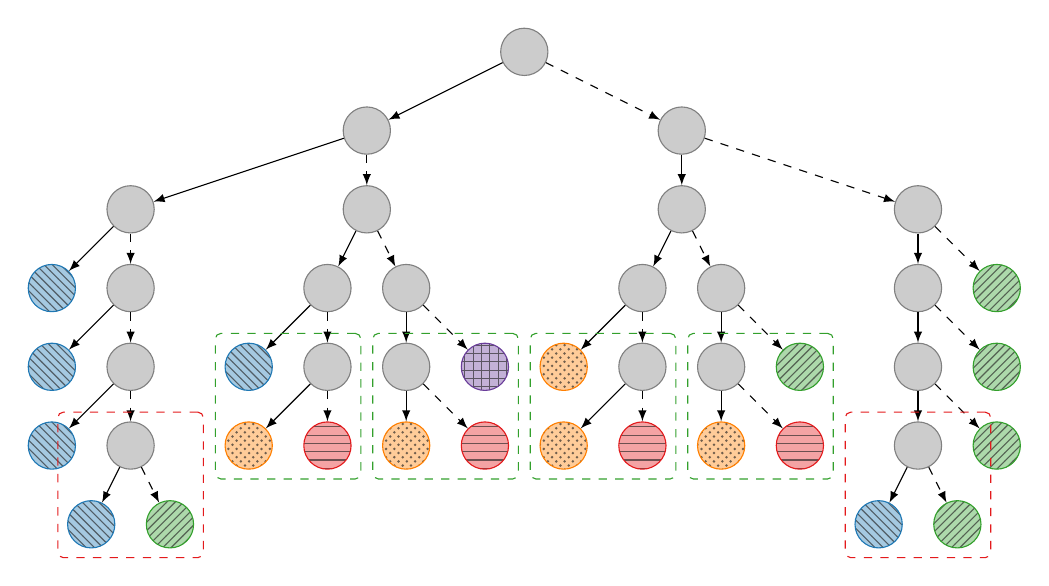
\begin{tikzpicture}[baseline]
    \node[any] (l0_n0)  at ( 6.5, 6.0) {};

    \node[any] (l1_n0)  at ( 4.5, 5.0) {};
    \node[any] (l1_n1)  at ( 8.5, 5.0) {};

    \draw[->,>=latex        ] (l0_n0) -- (l1_n0);
    \draw[->,>=latex, dashed] (l0_n0) -- (l1_n1);

    \node[any] (l2_n0)  at ( 1.5, 4.0) {};
    \node[any] (l2_n1)  at ( 4.5, 4.0) {};
    \node[any] (l2_n2)  at ( 8.5, 4.0) {};
    \node[any] (l2_n3)  at (11.5, 4.0) {};

    \draw[->,>=latex        ] (l1_n0) -- (l2_n0);
    \draw[->,>=latex, dashed] (l1_n0) -- (l2_n1);
    \draw[->,>=latex        ] (l1_n1) -- (l2_n2);
    \draw[->,>=latex, dashed] (l1_n1) -- (l2_n3);

    \node[r0 ] (l3_n0)  at ( 0.5, 3.0) {};
    \node[any] (l3_n1)  at ( 1.5, 3.0) {};
    \node[any] (l3_n2)  at ( 4.0, 3.0) {};
    \node[any] (l3_n3)  at ( 5.0, 3.0) {};
    \node[any] (l3_n4)  at ( 8.0, 3.0) {};
    \node[any] (l3_n5)  at ( 9.0, 3.0) {};
    \node[any] (l3_n6)  at (11.5, 3.0) {};
    \node[r1 ] (l3_n7)  at (12.5, 3.0) {};

    \draw[->,>=latex        ] (l2_n0) -- (l3_n0);
    \draw[->,>=latex, dashed] (l2_n0) -- (l3_n1);
    \draw[->,>=latex        ] (l2_n1) -- (l3_n2);
    \draw[->,>=latex, dashed] (l2_n1) -- (l3_n3);
    \draw[->,>=latex        ] (l2_n2) -- (l3_n4);
    \draw[->,>=latex, dashed] (l2_n2) -- (l3_n5);
    \draw[->,>=latex        ] (l2_n3) -- (l3_n6);
    \draw[->,>=latex, dashed] (l2_n3) -- (l3_n7);

    \node[r0 ] (l4_n0)  at ( 0.5, 2.0) {};
    \node[any] (l4_n1)  at ( 1.5, 2.0) {};
    \node[r0 ] (l4_n2)  at ( 3.0, 2.0) {};
    \node[any] (l4_n3)  at ( 4.0, 2.0) {};
    \node[any] (l4_n4)  at ( 5.0, 2.0) {};
    \node[spc] (l4_n5)  at ( 6.0, 2.0) {};
    \node[rep] (l4_n6)  at ( 7.0, 2.0) {};
    \node[any] (l4_n7)  at ( 8.0, 2.0) {};
    \node[any] (l4_n8)  at ( 9.0, 2.0) {};
    \node[r1 ] (l4_n9)  at (10.0, 2.0) {};
    \node[any] (l4_n10) at (11.5, 2.0) {};
    \node[r1 ] (l4_n11) at (12.5, 2.0) {};

    \draw[->,>=latex        ] (l3_n1) -- (l4_n0);
    \draw[->,>=latex, dashed] (l3_n1) -- (l4_n1);
    \draw[->,>=latex        ] (l3_n2) -- (l4_n2);
    \draw[->,>=latex, dashed] (l3_n2) -- (l4_n3);
    \draw[->,>=latex        ] (l3_n3) -- (l4_n4);
    \draw[->,>=latex, dashed] (l3_n3) -- (l4_n5);
    \draw[->,>=latex        ] (l3_n4) -- (l4_n6);
    \draw[->,>=latex, dashed] (l3_n4) -- (l4_n7);
    \draw[->,>=latex        ] (l3_n5) -- (l4_n8);
    \draw[->,>=latex, dashed] (l3_n5) -- (l4_n9);
    \draw[->,>=latex        ] (l3_n6) -- (l4_n10);
    \draw[->,>=latex, dashed] (l3_n6) -- (l4_n11);

    \node[r0  ] (l5_n0)  at ( 0.5, 1.0) {};
    \node[any ] (l5_n1)  at ( 1.5, 1.0) {};
    \node[rep ] (l5_n2)  at ( 3.0, 1.0) {};
    \node[spc4] (l5_n3)  at ( 4.0, 1.0) {};
    \node[rep ] (l5_n4)  at ( 5.0, 1.0) {};
    \node[spc4] (l5_n5)  at ( 6.0, 1.0) {};
    \node[rep ] (l5_n6)  at ( 7.0, 1.0) {};
    \node[spc4] (l5_n7)  at ( 8.0, 1.0) {};
    \node[rep ] (l5_n8)  at ( 9.0, 1.0) {};
    \node[spc4] (l5_n9)  at (10.0, 1.0) {};
    \node[any ] (l5_n10) at (11.5, 1.0) {};
    \node[r1  ] (l5_n11) at (12.5, 1.0) {};

    \draw[->,>=latex        ] (l4_n1)  -- (l5_n0);
    \draw[->,>=latex, dashed] (l4_n1)  -- (l5_n1);
    \draw[->,>=latex        ] (l4_n3)  -- (l5_n2);
    \draw[->,>=latex, dashed] (l4_n3)  -- (l5_n3);
    \draw[->,>=latex        ] (l4_n4)  -- (l5_n4);
    \draw[->,>=latex, dashed] (l4_n4)  -- (l5_n5);
    \draw[->,>=latex        ] (l4_n7)  -- (l5_n6);
    \draw[->,>=latex, dashed] (l4_n7)  -- (l5_n7);
    \draw[->,>=latex        ] (l4_n8)  -- (l5_n8);
    \draw[->,>=latex, dashed] (l4_n8)  -- (l5_n9);
    \draw[->,>=latex        ] (l4_n10) -- (l5_n10);
    \draw[->,>=latex, dashed] (l4_n10) -- (l5_n11);

    \node[r0] (l6_n0) at ( 1.0, 0.0) {};
    \node[r1] (l6_n1) at ( 2.0, 0.0) {};
    \node[r0] (l6_n2) at (11.0, 0.0) {};
    \node[r1] (l6_n3) at (12.0, 0.0) {};

    \draw[->,>=latex        ] (l5_n1)  -- (l6_n0);
    \draw[->,>=latex, dashed] (l5_n1)  -- (l6_n1);
    \draw[->,>=latex        ] (l5_n10) -- (l6_n2);
    \draw[->,>=latex, dashed] (l5_n10) -- (l6_n3);

    \node[draw=Paired-5, rounded corners=2pt, dashed, fit=(l5_n1) (l6_n0) (l6_n1)] {};
    \node[draw=Paired-5, rounded corners=2pt, dashed, fit=(l5_n10) (l6_n2) (l6_n3)] {};

    \node[draw=Paired-3, rounded corners=2pt, dashed, fit=(l4_n3) (l5_n2) (l5_n3)] {};
    \node[draw=Paired-3, rounded corners=2pt, dashed, fit=(l4_n4) (l5_n4) (l5_n5)] {};
    \node[draw=Paired-3, rounded corners=2pt, dashed, fit=(l4_n7) (l5_n6) (l5_n7)] {};
    \node[draw=Paired-3, rounded corners=2pt, dashed, fit=(l4_n8) (l5_n8) (l5_n9)] {};
  \end{tikzpicture}
\end{document}